\newcommand{\hsmasprache}{en} 

\input{preambel}

% Titel der Arbeit auf Deutsch
\newcommand{\hsmatitelde}{Konzeption, Implementierung und Evaluation eines Machbarkeitsnachweises eines modularen Proxys zum Testen von Anwendungen im Internet der Dinge}

% Titel der Arbeit auf Englisch
\newcommand{\hsmatitelen}{Conception, Implementation, and Evaluation of a Proof of Concept of a Modular Proxy Application for Testing Internet of Things Applications}

% Weitere Informationen zur Arbeit
\newcommand{\hsmaort}{Mannheim}    % Ort
\newcommand{\hsmaautorvname}{Moritz Laurin} % Vorname(n)
\newcommand{\hsmaautornname}{Thomas} % Nachname(n)
\newcommand{\hsmadatum}{31.05.2021} % Datum der Abgabe
\newcommand{\hsmajahr}{2020} % Jahr der Abgabe
\newcommand{\hsmafirma}{NVISO GmbH, Frankfurt} % Firma bei der die Arbeit durchgeführt wurde
\newcommand{\hsmabetreuer}{Prof. Dr. Thomas Specht, Hochschule Mannheim} % Betreuer an der Hochschule
\newcommand{\hsmazweitkorrektor}{Pierre-Alain Mouy, M.Sc., NVISO GmbH} % Betreuer im Unternehmen oder Zweitkorrektor
\newcommand{\hsmafakultaet}{I} % I für Informatik oder E, S, B, D, M, N, W, V
\newcommand{\hsmastudiengang}{IM} % IB IMB UIB CSB IM MTB (weitere siehe titleblatt.tex)

% Zustimmung zur Veröffentlichung
\setboolean{hsmapublizieren}{true}   % Einer Veröffentlichung wird zugestimmt
\setboolean{hsmasperrvermerk}{false} % Die Arbeit hat keinen Sperrvermerk

% -------------------------------------------------------
% Abstract
% Achtung: Wenn Sie im Abstrakt Anführungszeichen verwenden wollen, dann benutzen Sie
%          nicht "` und "', sondern \enquote{}. "` und "' werden nicht richtig
%          erkannt.

% Kurze (maximal halbseitige) Beschreibung, worum es in der Arbeit geht auf Deutsch
\newcommand{\hsmaabstractde}{Als Konsequenz der voranschreitenden Digitalisierung werden ehemals analoge Geräte zunehmend digitalisiert und somit Teil des \enquote{Internets der Dinge} (\enquote{Internet of Things}, IoT). Dabei stellt jedoch die große Bandbreite an Anwendungen eine potenziell große Angriffsfläche für Angreifer dar. Um diesem Risiko, das die sogenannten \enquote{smarten} Anwendungen gegenüber ihren Betreibern darstellen, zu begegnen, untersuchen und überprüfen Sicherheitsforscher und Penetrationtester deren Sicherheitsarchitekturen. Daraus erwächst ein Bedarf an einer modularen Proxy-Anwendung, die sie dabei unterstützt, die heterogene Verwendung von Kommunikationsprotokollen in IoT-Anwendungen zu beherrschen. Ziel dieser Arbeit ist die Konzeption eines Softwareentwurfs für eine solche Anwendung und deren prototypische Umsetzung sowie eine Bewertung ihrer Nützlichkeit. Quantitative Ergebnisse sind die Dokumentation des Problemstellung, ein abstraktes Entwurfskonzept und eine Reihe von Herausforderungen bei der Entwicklung sowie daraus gewonnene Erkenntnisse.} 

% Kurze (maximal halbseitige) Beschreibung, worum es in der Arbeit geht auf Englisch
\newcommand{\hsmaabstracten}{Today, more and more formerly analogue physical entities are now being digitized and connected to the internet, adding to the \enquote{Internet of Things}. However, the wide variety in appliances poses a potentially wide attack surface for malicious actors. To address this risk that these so-called smart devices pose to parties that employ them, security researchers and penetration testers examine and test their security implementation. The need arises for a modular proxy application that allows to test the heterogeneous landscape of communication protocols used in IoT applications. The goal of this thesis is to conceptualize a design for such an application, realize a prototypic implementation thereof and evaluate its usefulness. Quantitative results are a documentation of the problem space, an abstract design concept and sets of development challenges and lessons learned. }  

\addbibresource{literature.bib}   

\begin{document}
\frontmatter

\setcounter{page}{0}
\changefont{ptm}{m}{n}  
\renewcommand{\rmdefault}{ptm}

\input{titelblatt}

\cleardoublepage
\pdfbookmark{\contentsname}{Contents}
\tableofcontents

\cleardoublepage
\newcounter{frontmatterpage}
\setcounter{frontmatterpage}{\value{page}}

\mainmatter

\onehalfspacing

\chapter{Introduction}

\section{Motivation}
Test\cite{Ledwaba2019}
\section{Purpose and Structure of the Thesis}
% 2. Verwandte Arbeiten
\chapter{Related Work}
\label{chap:related-work}

As part of their master's thesis, Bellemans conducted a study in 2020 that evaluated the security and privacy implementations of fifteen \enquote{\emph{smart}} devices from a wide price range available on the market at the time. They performed automated analyses and requested data access from manufacturers \cite{JonahBellemans}. The thesis showed that the devices made use of a variety of both standardized and proprietary transport and application protocols. It also found severe flaws in the devices' compliance to \ac{GDPR}: about one third of the devices' manufacturers did not reply to \ac{GDPR} requests at all, however Bellemans noted that the COVID-19 pandemic may have had an impact on their data access requests. The thesis suggests that the introduction of a quality label that guarantees appropriate implementation of security and privacy aspects could prove beneficial for customers. \par
In 2017, Apthorpe et al. presented a three stage strategy to examine metadata of network traffic of four smart devices \cite{apthorpe2017smart}.
By monitoring the devices' traffic, they showed that even though the communication between the devices and their corresponding internet servers were encrypted, passive observers could deduce information about users' behaviour by identification of the destination server and analysis of the rate of traffic being sent. A noteworthy aspect of their work is that they performed this analysis from an \ac{ISP}'s point of view, exclusively examining metadata of the communication that took place. The strategy described in the paper consists of the following (greatly simplified) steps:
\begin{enumerate}
    \item Identifying communication streams of individual devices (e.g. by examining the TCP packets' destination IPs).
    \item Associating the streams with specific device models (e.g. by performing reverse-look ups of the aforementioned IPs).
    \item Analysing traffic rates (presuming that traffic is generated upon taking measures).
\end{enumerate}


Apthorpe et al. conclude that their strategy works well on inferring behaviour from regular internet traffic of smart devices, however they suppose that shaping traffic or making use of proxies (that effectively mask the destination IPs) could be effective counter-measures. It is safe to assume that regular smart home setups do not make use of proxies or traffic shaping though, thus being vulnerable to this kind of attack. 
\chapter{Theoretical Background}
\label{chap:theoretical-background}
This chapter provides an overview of the technologies and concepts referred to in subsequent chapters.
Starting with section \ref{sec:computer-networks}, essential concepts of computer communication in networks will be presented and examined, covering the concept of network layers, intercepting of communication between two parties and analysis of transferred data.
Building upon these fundamentals, section \ref{sec:internet-of-things} introduces the fields of use of \ac{IoT} applications, common architectures used today to implement them and popular protocols they make use of. Lastly, it will discuss security considerations important to \ac{IoT} applications.
After that, section \ref{sec:information-security} will provide insights into relevant concepts and the practices used and applied in information security. It covers key concepts and legal considerations, integration of information security in software development and common practices and methods involved. %TODO: Update


\section{Design Patterns}
\subsection{Pipeline/Pipes and Filters Pattern}
In a paper from 1996, Alencar et al. describe the pipes and filters pattern as a mechanism to process streams of data \cite{alencar_cowan_lucena_1996}. They state that the pattern features \enquote{pipes} and \enquote{filters} components: pipes relay data streams between filters while the filters process the data streams' contents. Figure \ref{fig:dp-pipes-filters} shows an exemplaric sequence of $n$ pipes and filters relaying and processing an object $O$ by implementing pipes as method calls. Alencar et al. state that the pattern's \enquote{objective is to obtain highly reusable, interchangeable and maintainable applications}.
\begin{figure}[h!]
    \centering
    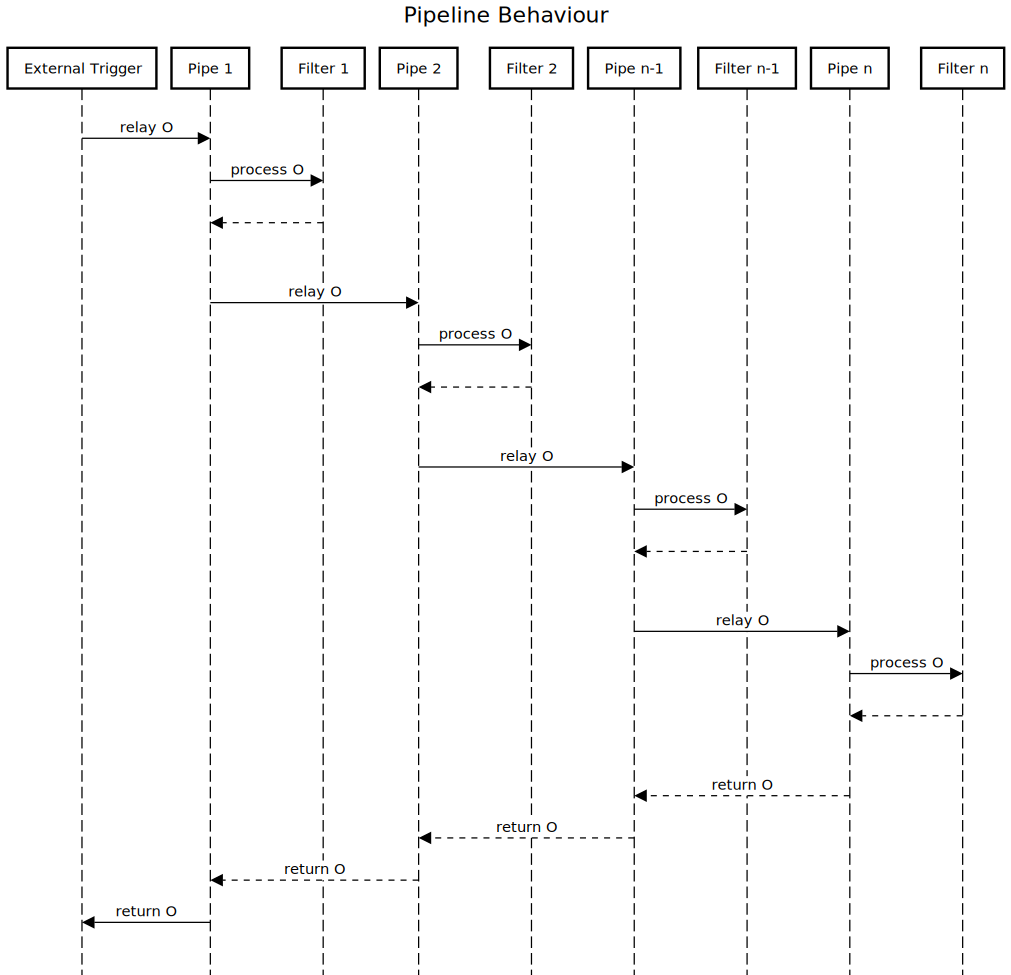
\includegraphics[width=14cm]{img/ch03/pipeline-behaviour.pdf}
    \captionof{figure}{?} % TODO: Describe
    \label{fig:dp-pipes-filters}
\end{figure}
\subsection{Abstract Factory/Kit Pattern}
Gamma et al. describe the intent of the abstract factory pattern as follows: "provide an interface for creating families of related or dependent objects without specifying their concrete classes" \cite{Gamma1998}. They propose the following components:
\begin{itemize}
    \item \enquote{AbstractProduct}: interface for products.
    \item \enquote{AbstractFactory}: interface for creating objects that implement \enquote{AbstractProduct}.
    \item \enquote{ConcreteProduct}: classes that implement \enquote{AbstractProduct}.
    \item \enquote{ConcreteFactory}: classes that implements \enquote{AbstractFactory} and create \enquote{ConcreteProducs}. 
\end{itemize}
They conclude that there are multiple consequences to using the pattern, one being that it \enquote{isolates concrete classes}, meaning that there is a clear isolation from the Client and the ConcreteFactories.
%CITE: 1996 Paper Design Patterns in Software Design Patterns
%CITE: 1997 - Book - Design Patterns
\subsection{Publish-Subscribe/Observer Pattern}
%CITE: 1997 - Book - Design Patterns
In their book \enquote{Design Patterns - Elements }, Gamma et al.
\section{Computer Communication}
\label{sec:computer-networks}
\emph{TBD: OSI-Modell} %TODO
%CITE: ISO/IEC 1994
%TBD: Proxy?

\section{(Industrial) Internet of Things}
\label{sec:internet-of-things}
\subsection{Fields of Use}
%TBD: KRITIS
%CITE: 2013 - Book - BSI
%Smart Home?
\subsection{Application Architectures}
\emph{TBD: Cloud + Device}
\subsection{Common Protocols}
\label{sec:iot-common-protocols}
Building up on pre-existing network infrastructure and in order to meet requirements specific to individual fields of use and use-case scenarios, the landscape of \ac{IoT} attends with a great variety of \emph{communication protocols} (further used to refer to both transport and application protocols). This section will provide a brief overview of the working principles, use cases and history of some protocols commonly used in \ac{IoT} and \ac{IIoT} applications today.
\paragraph{\ac{HTTP}} \emph{TBD} %TODO
\ac{HTTPS}
%CITE: 1.0 https://datatracker.ietf.org/doc/html/rfc1945
%CITE: 2019 - Book - SmartInnovationsInCommunicatio - p174
\paragraph{\ac{WS}} \emph{TBD}

%CITE: https://datatracker.ietf.org/doc/html/rfc6455
%CITE: PMCE https://tools.ietf.org/html/rfc7692
\paragraph{\ac{MQTT}}
\cite{gupta_banks_2015}

\paragraph{Industrial} Modbus \ac{TCP}, Profibus/Profinet, \ac{OPC U/A}

\section{Information Security}
\label{sec:information-security}
\subsection{The CIA Triad}

\subsection{Methodology}
\subsubsection{Penetration Testing}
\subsubsection{Red-Teaming}
\subsubsection{Fuzzing}

\subsection{Man-In-The-Middle Attacks}
\ac{MITM}
%Cite: A Survey of Man In The Middle Attacks

\subsection{Tools}
There are many tools used in information security. They vary greatly in their features, field of use and maturity. The following paragraphs describe tools relevant to this thesis and the fields of use it touches.

\paragraph{Wireshark} First released in 1998, \emph{Wireshark} is a cross-platform and open-source tool used for network analysis, including \emph{network sniffing} \cite{wireshark}. It is written mainly in C, consists of more than 3,600,000 lines of C code\footnote{This number was returned by the \emph{cloc} utility run on commit \emph{c73ab16b} from 23rd May 2021 of Wireshark's GitLab source-code repository \cite{wiresharkgit}.} and features a \ac{GUI}. Although it is described as a network protocol analyser, it also supports sniffing of \ac{USB} packets. It implements a wide array of \emph{dissectors} for various protocols and allows detailed examination of network packets (as shown in figure \ref{fig:wireshark}).

\begin{figure}[h]
    \centering
    \includegraphics[width=14cm]{img/ch03/wireshark.png}
    \captionof{figure}{Screenshot of Wireshark being executed and dissecting a \ac{HTTP} $GET$ request to the site \enquote{httpbin.org}. The display-filter \enquote{tcp.port == 80} shows only packets sent to or from port 80 (e.g. \ac{HTTP} communication).}
    \label{fig:wireshark}
\end{figure}

\subsubsection{Specific \acp{MITM}}
The following tools are \acp{MITM} that support specific protocols only:
%Specific mitms:
\paragraph{Burp Suite} Developed and distributed by \enquote{PortSwigger} as a commercial product, \emph{Burp Suite} is a tool specialized for web-application testing \cite{burpsuite}. It can be used as a \ac{MITM} for \ac{HTTP} communication by configuring the operating system or browser to use its internal \ac{HTTP} server as a proxy. While it implements basic support for \ac{WS}, it is mainly used for \ac{HTTP} (and nowadays \ac{HTTPS}) and lacks support for other protocols. Aside from its internal proxy server, it also provides specialized features such as the \enquote{Repeater} which is used to send forged \ac{HTTP} requests. The freely available \enquote{Community Edition} (shown in figure \ref{fig:burpsuite}) allows use of most of the tool's features.

\begin{figure}[h]
    \centering
    \includegraphics[width=14cm]{img/ch03/burpsuite.png}
    \captionof{figure}{Screenshot of Burp Suite being used to send forged \ac{HTTP} requests to the site \enquote{httpbin.org}.}
    \label{fig:burpsuite}
\end{figure}
\paragraph{mitmproxy} %focused on HTTP/S + WS but supports extension, largely undocumented source
\paragraph{mProxy}
\paragraph{IOXY}
%Generic
\subsubsection{Generic \acp{MITM}}
The following tools are generic \acp{MITM} that support a wide range of network protocols:
\paragraph{ettercap} While \emph{ettercap} was initially developed as a network sniffer for switched \ac{LAN}, it was gradually extended to implement a set of \ac{MITM} attacks such as \ac{ARP} spoofing and \emph{packet filtering} which allowed modifying intercepted communication \cite{ettercap}. Penetration testers can write custom filters in a scripting language to implement their own packet filtering logic. It is written in C and implements network protocols of layers 1 to 4 of the \ac{OSI} model. Thus, it does not implement application protocols.
\paragraph{bettercap} Similar to ettercap, \emph{bettercap} implements network sniffing and other features used for network analysis and discovery. However, contrary to ettercap, it aims to support a wider range of transport technologies and is described as \enquote{\emph{the Swiss Army knife for WiFi, Bluetooth Low Energy, wireless HID hijacking and IPv4 and IPv6 network reconnaissance and MITM attacks}} \cite{bettercap}. It is written in Go and features a web-interface for configuration, control and monitoring.
\paragraph{Scapy}
\paragraph{MITMf} %Built on scapy, implements some attacks and servers, not maintained anymore, superseded by bettercap 
%4. Problemraum (Prototyp, Testaufbauten, bestehende Software)
\chapter{Understanding the Problem Space}
\label{chap:understanding-the-problem-space}
In order to provide a satisfying solution to the problem at hand, the problem itself and the environment it occurs in must be researched. This chapter aims to explore and examine the problem space, resulting in a set of artifacts (namely a domain model and a set of requirements) that aid in understanding the context and designing an appropriate solution. First, a prototypical network proxy is designed and implemented in section \ref{sec:prototypical-implementation} to get an understanding of the problems and challenges involved in designing, implementing and using such software. Based on these experiences, interviews with experts in penetration testing are conducted and evaluated in section \ref{sec:interviews} to get a proper understanding of their everyday work and resulting problems. Lastly, existing software that aims to intercept communication for various scenarios and technologies is examined in section \ref{sec:analysis-existing-software}, compared to each other and their usefulness for the problem-specific scenarios is assessed.

\section{Prototypical Implementation}
\label{sec:prototypical-implementation}
The prototype was designed to be able to handle two scenarios; a simple and a complex one. Complexity was evaluated by the amount of communication protocols and steps involved. The goal of this section was to implement a prototype that could be used to intercept communication between an \ac{IoT} device and its cloud service as shown in figure \ref{fig:network-communication-diagrams}.   

\begin{figure}%
    \centering
    \subfloat[\centering Regular communication between an \ac{IoT} device and a cloud service.]{{\includegraphics[width=10cm]{img/ch04/Setup - 1 Regular.pdf} }}%
    \qquad
    \subfloat[\centering Communication intercepted by a \ac{MITM} proxy.]{{\includegraphics[width=10cm]{img/ch04/Setup - 2 Pentesting.pdf} }}%
    \caption{Installing a \ac{MITM} proxy to intercept network communication for penetration testing.}%
    \label{fig:network-communication-diagrams}%
\end{figure}

\subsection{Simple Scenario: ICS Modbus TCP}
% Hardware Setup
% Communication

\subsection{Complex Scenario: AWS IoT}
% Hardware Setup
% Communication



\subsection{Requirements}
%TODO: Move overscoped requirements to design of the second prototype?
To be able to operate in both of the aforementioned scenarios, the prototype had to implement a set of functional requirements:
\begin{itemize}
    \item [\textbf{F1}] \textbf{Protocols:} The software must implement parsing/crafting messages/packets of the following communication protocols: \ac{HTTP}, \ac{WS}, \ac{MQTT} and Modbus \ac{TCP}. \\
    \textit{Fit criterion: TBD} %TODO: Do lol 
    \item [\textbf{F2}] \textbf{Network Stacks:} The software must provide an interface to the user where they can specify which communication protocols are to be used and whether and how they are stacked (further referred to as \emph{network stack}).\\
    \textit{Fit criterion: The software processes a configuration file that lets users specify which protocols to be used and whether/how they are stacked.} 
    \item [\textbf{F3}] \textbf{State Machine:} The software must provide an interface for the user to specify when to switch to using another network stack, represented using state machines.\\
    \textit{Fit criterion: The software processes a configuration file that lets users specify when to switch between network stacks.}
    \item [\textbf{F4}] \textbf{Integration:} The software shall provide interfaces for integration of third-party software.\\
    \textit{Fit criterion: The software allows sending requests/responses to \enquote{Burp Suite} for manipulation.} %TODO: Do lol
    \item [\textbf{F5}] \textbf{Scripting:} The software shall provide scripting capabilities for automated manipulation of messages/packets.\\
    \textit{Fit criterion: Users can define script-snippets to be executed on messages/packets.} %TODO: Do lol
\end{itemize}

The following non-functional requirements were defined:

\begin{itemize}
    \item [\textbf{N1}] \textbf{Extensibility:} To allow for future implementation of further communication protocols the software shall be implemented in a modular fashion.
    \item [\textbf{N2}] \textbf{Platform Compatibility:} In order to support a broad spectrum of target platforms, the software shall be implement plattform-independently.
\end{itemize}

Due to this implementation serving as a prototype and being of an academic nature, no specific constraints were defined. It was developed strictly ignoring aspects of usability and stability as it should not be used in production environments but in laboratories exclusively.

\subsection{Design}
% Overall
% Network Stack
\begin{figure}[t]
    \centering
    \includegraphics[width=6cm]{img/ch04/Architecture - Pipes and Filters.pdf}
    \captionof{figure}{Statemachine of \ac{AWS} \ac{IoT} communication}
    \label{fig:aws-statemachine}
\end{figure}

% TODO: References Pipes & Filters \ref{fig:app-diag-pipesfilters-1} \ref{fig:app-diag-pipesfilters-2}

% Statemachine
\begin{figure}[t]
    \centering
    \includegraphics[width=6cm]{img/ch04/Statemachine 2.pdf}
    \captionof{figure}{Statemachine of \ac{AWS} \ac{IoT} communication}
    \label{fig:aws-statemachine}
\end{figure}
% Reference: https://aws.amazon.com/blogs/aws/aws-iot-cloud-services-for-connected-devices/


\subsection{Implementation}

\subsection{Insights Gained}


%\begin{figure}[t]
%    \centering
%    \includegraphics[width=6cm]{img/ch04/Architecture - Simple.pdf}
%    \captionof{figure}{High-level Software Architecture}
%    \label{fig:high-level-software-architecture}
%\end{figure}

%\begin{figure}[t]
%    \centering
%    \includegraphics[width=6cm]{img/ch04/Architecture - Pipes and Filters.pdf}
%    \captionof{figure}{"Pipes and Filters" Design Pattern}
%    \label{fig:design-pattern-pipes-and-filters}
%\end{figure}



\emph{TBD; implementation is completed, needs to be written down; include its diagrams} %TODO

\section{Interviewing Experts for Insights}
\label{sec:interviews}
Interviews may be an efficient way to get an expert’s opinion on something they are a professional in. Thus, expert interviews were conducted to let security researchers give insight into their everyday work and the challenges they face. The information and insights gathered in these interviews were then used to model a persona, various work scenarios and use-cases that as a whole aim to represent their work.

\subsection{Interview Guideline}
An interview guideline (shown in \emph{TBD}) %TODO: Reference appended interviews
was created to keep focus on key points during interviews so that interviewees would not stray too far from the relevant points. The guideline also served as a checklist so the interviewer could make sure that all questions and points that should be covered  initially, were in fact covered by the end of the interviews. It was composed of three sections:

\paragraph{1. Experiences with IoT} The answers to these questions would give insights into what kind of applications the security researchers had worked on in the past. Answers to question \emph{1.1.} were of particular interest as they might represent what technologies were being examined by security researchers and may be popular in today’s applications.
\paragraph{2. Processes in Everyday Life} This section aimed to cover questions about the processes and tasks security researchers perform during penetration tests of IoT applications in their everyday life. Ideally, answers to those questions would show the approaches taken and challenges faced during their work, uncovering potential needs and underlying motivation.
\paragraph{3. The Future of IoT} This section had security researchers assess what the future of IoT may be like from their point of view. This required the interviewees to make a critical assessment of the status quo.

%The experience gained from implementing the prototype in \ref{sec:prototypical-implementation} greatly influenced the creation of this guideline. For example question \emph{1.3. Were there any special constrains (e.g. real-time systems) when working with them?} 

%Some of the questions in these sections originated from or were influenced by experience gained when implementing the prototype proxy application in \ref{sec:prototypical-implementation}. 

\subsection{Conducting Interviews}
Interviews were conducted with six %Patrick, Cédric, Théo, Oliver, Pierre
\emph{NVISO} employees that all had worked on security assignments on \ac{IoT} or \ac{IIoT} applications in the past. There is considerable variety in
\begin{itemize}
    \item the experience they had in working on security assignments in general: all interviewees had a strong background in cyber security that reached back multiple years except one who was a working student at \emph{NVISO Labs}.
    \item and the experience they had in working on \ac{IoT}/\ac{IIoT} applications: two interviewees worked on assessing \ac{IoT}/\ac{IIoT} applications only occasionally, one was part of a car manufacturer's automotive security team and three were part of \emph{NVISO Labs} and worked with smart devices on a regular basis.
    % Position? CEO vs. Consultant vs. Werkstudent
    % 
\end{itemize}
The duration of the interviews varied from 45 minutes to two hours depending on the amount and level of detail of information provided by the interviewees and the number of times that the interviewer had to ask further questions.

\emph{TBD: Summary of the interviews and conclusions drawn + personas and use cases}

\section{Analysis of Existing Software}
\paragraph{Wireshark} 3,690,000 lines of code\footnote{This number was returned by the \emph{cloc} utility run on commit \emph{3a8111e1c2adcdc0603993c6ed5d20a40f162125} of Wireshark's Github mirror.}\emph{TBD}
\paragraph{MITMf} \emph{TBD}
\paragraph{Ettercap} \emph{TBD}
\paragraph{bettercap} \emph{TBD}
\paragraph{mitmproxy} \emph{TBD}
\paragraph{mProxy} \emph{TBD}
\paragraph{IOXY} \emph{TBD}

\emph{TBD; planned: paragraph about each program including a general description, uses, capabilities and usefulness} %TODO
\label{sec:analysis-existing-software}
\begin{table}[h]
    \centering
    \begin{tabular}{r|c|c|c|c|c|c}
        \toprule
              \thead{$Name$} & \thead{$Latest$\\$Release$} & \thead{$Implemented$\\$in$} & \thead{$Supported$\\$Protocols$} & \thead{$R$} & \thead{$W$} & \thead{$D$}\\
        \midrule
            Wireshark & 2020-07-01 & C & Various & \cellcolor{green!25}Y & \cellcolor{red!25}N & \cellcolor{red!25}N \\
        \midrule
            MITMf & 2015-08-28 & Python & Various & ? & \cellcolor{green!25}Y & \cellcolor{green!25}Y  \\ %https://github.com/byt3bl33d3r/MITMf
        \midrule
            Ettercap & 2019-07-01 & C & Various & \cellcolor{green!25}Y & \cellcolor{green!25}Y & \cellcolor{green!25}Y  \\
        \midrule
            bettercap & 2020-03-13 & Go & Various & \cellcolor{green!25}Y & \cellcolor{green!25}Y  & \cellcolor{green!25}Y \\
        \midrule
            mitmproxy & 2020-03-13 & Python & HTTP/S, WS & \cellcolor{orange!25}P & \cellcolor{orange!25}P & \cellcolor{orange!25}P \\ %https://github.com/mitmproxy/mitmproxy
        \midrule
            mProxy & Pre-Releases only & Go & MQTT & ? & \cellcolor{green!25}Y & - \\ %https://github.com/mainflux/mproxy
        \midrule
            IOXY & Source only & Go & MQTT & \cellcolor{green!25}Y & \cellcolor{green!25}Y & \cellcolor{green!25}Y \\ %https://github.com/mainflux/mproxy
        \bottomrule
    \end{tabular}
    \caption[Comparison of existing software]{Comparison of existing software where $R$, $W$ and $D$ describe read, write and deletion capabilities, respectively. $Y$, $N$ and $P$ indicate full, no or partial functionality, respectively.}
    \label{table:comparison-existing-software}
\end{table}
% 4. Konzept (Kontext, Ablauf, Anforderungen [Interviews], Konzept [Architektur])
\chapter{Conceptual Design}
\label{chap:conceptual-design}
%This chapter will detail the process of conceptualizing the design of the modular proxy application based on the results of the preceding chapter. First, the requirements are analysed for their potential design implications in section \ref{sec:req-design-implications}. Afterwards the user interactions and domain entities identified in chapter \ref{chap:understanding-the-problem-space} are examined and broken down into communication flows between actors and systems in section \ref{sec:user-interactions-designing-workflow} and individual software components that complete the design are discussed in section \ref{sec:inferring-software-components}. Lastly, an overview of the complete design concept is given in section \ref{sec:abstract-design-concept}, discussing potential advantages and constraints. %TODO: Rewrite & update

%\section{Inferring Software Components}
%\label{sec:inferring-software-components}
Building on the software design of the first prototype presented in section \ref{sec:prototype-design} and the insights gained in section \ref{sec:prototype-insights}, two design concepts were worked out. The following sections will detail components and principles of both concepts.

\section{Design \#1: Singular Proxy Application}
This design concept is based on the general ideas presented in section \ref{sec:prototype-design} (e.g. state-machines, network stacks and pipes) and employs a basic architecture shown in figure \ref{fig:component-view-1}.\\
\begin{figure}[h]
    \centering
    \includegraphics[width=12cm]{img/ch05/component-view-1.pdf}
    \captionof{figure}{High-level component diagram of the proxy application concept}
    \label{fig:component-view-1}
\end{figure}
As discussed in the previous chapter, the requirement \enquote{F2 Network Stacks} introduces the need for dynamically initialized objects which in this concept is implemented by making use of the factory pattern in the \enquote{Site} component. This component allows for registering \emph{Factories} that are used to initialize objects. Similar to the implementation in the first prototype, factories initialize objects using metadata supplied from a configuration file.\\
Communication with other systems is encapsulated into the \enquote{Message IO}-package shown in figure \ref{fig:component-view-2}. Applications that are tested by penetration testers are connected to sockets provided by the \enquote{Gateway} component and temporarily stored in a message queue to be processed by the network stacks organized by the \enquote{Global Statemachine}. Similar to the \enquote{Server} interface used in the first prototype, gateways provide means of communicating with external systems and receiving and sending messages. They are highly abstract and meant to be used for implementing interfaces for any kind of communication protocols and technologies, such as \ac{IP}-based \ac{TCP} and \ac{UDP} communication but also other protocols such as USB, Bluetooth, ZigBee or KNX.
\begin{figure}[h]
    \centering
    \includegraphics[width=12cm]{img/ch05/component-view-2-messageio.pdf}
    \captionof{figure}{The \enquote{Message IO}-package}
    \label{fig:component-view-2}
\end{figure}
It should be noted that the static view of the design is rather simple due to its dynamic runtime behaviour: many instances and relationships are only instantiated at runtime and not pre-determined. An schematic representation of the dynamic structure and interweaving of state-machines, network stacks and pipes (in this concept called a \enquote{pipeline}) is shown in figure \ref{fig:pipeline}. This figure highlights a series of active state-machines and network stacks which together constitute the active pipeline. \\
Figure \ref{fig:app-activity-fsms} illustrates the recursive nature of this concept processing (dequeued) messages:
\begin{enumerate}
    \item A state-machine $F$ (initialized with the global state-machine instance) relays messages $M$ through its active state $S$'s network stack instance $N$.
    \item In $N$, all of its pipes $P$ process $M$ until the end of $N$ is reached ($P$ does not hold a reference to a succeeding pipe instance). If $F$ holds a reference to a succeeding \ac{FSM}, $F$ is set to this reference and the processes continues from step $1$.
    \item If $N$ does not hold a reference to a nested \ac{FSM}, the end of the network stack is reached and the direction of traversing the network stack is reversed.
    \item $P$ is set to $N$'s last pipe instance and $M$ is processed by $P$ until the start of $N$ is reached (i.e. $P$ does not hold a reference to a preceding pipe instance). If $F$ holds a reference to a preceding \ac{FSM} instance, $F$ is set to this reference, $N$ is set to $F$'s network stack reference and the process continues from step $4$.
    \item If $N$ does not hold a reference to a preceding \ac{FSM}, the beginning of the whole pipeline is reached and $F$ is the global state-machine.
\end{enumerate}

\begin{figure}[h]
    \centering
    \includegraphics[width=14cm]{img/ch05/classes-1-fsm-rules-netstack.pdf}
    \captionof{figure}{?} %TODO: Describe
    \label{fig:classes-1-fsm-rules-netstack}
\end{figure}
\paragraph{State-Machines} The classes related to the state-machine component are shown in figure \ref{fig:classes-1-fsm-rules-netstack}: \emph{StateMachines} hold a set of \emph{States} and \emph{Transitions}. In order to change states, state-machines evaluate a context by checking each of their transitions for whether their conditions for transition are met or not. This context is an aggregation of the \emph{memory} of each state-machine and their active states in the active pipeline. Transitions are defined by a source state, destination state and an \emph{IRule} that evaluates a given context. Rules can be concatenated with logical $AND$ or $OR$ operators and are designed to be scripts that operate on the given context. This allows the creation of nested rules such as the following one:
\begin{align*}
    \mathbf{changeToWS}(c) & = \mathbf{AND}(\mathbf{clientUpgrade}(c), \mathbf{serverUpgrade}(c))
\end{align*}
In this example, a transition with the above rule would evaluate to $true$ and trigger a state transition in a state-machine when the aggregated memory $c$ of all state-machines and their active states of the active pipeline indicated that an \ac{HTTP} request was detected that requested an upgrade to the \ac{WS} protocol (for instance, $clientUpgrade$ would look for an entry $clientUpgradeRequested$ in $c$ and evaluate its contents) and that an \ac{HTTP} response was detected that confirmed the upgrade request. This would allow a state-machine to detect upgrades of \ac{HTTP} communication to the \ac{WS} protocol.\\
States hold a \emph{NetStack} which in turn encapsulate a series of connected pipes, holding references to this series' first and last elements.
\begin{figure}[h]
    \centering
    \includegraphics[width=14cm]{img/ch05/classes-3-gateway.pdf}
    \captionof{figure}{?} %TODO: Describe
    \label{fig:classes-3-gateway}
\end{figure}
\paragraph{Gateway} The gateway component is implemented as the \enquote{GatewayPipe} (shown in figure \ref{fig:classes-3-gateway}). Improving on the first prototype's design, the GatewayPipe acts as a multiplexing pipe that accepts messages originating from two \enquote{RelayPipes} that act as two communication ports (e.g. the client device and the cloud server of scenario \#2 described in section \ref{sec:example-scenarios}) that hold information about the address of their communication peers in their address field (e.g. an \ac{IP} address of the remote peer). For instance, two \ac{TCP} client sockets can be handled by two \enquote{TcpPipes} (that inherit from the RelayPipe class), allowing \ac{TCP} packets to be routed into the pipeline via a GatewayPipe.
\paragraph{Pipes} Building upon the approach of routing and processing messages via pipes discussed in section \ref{sec:prototype-design}, this design concept addresses some inconsistencies of the former design and adds needed flexibility. As shown in figure \ref{fig:app-classes-2-pipes}, the \enquote{IPipe} interface persisted and is extended by the \enquote{ITrackablePipe} interface that adds a unique identifier to pipes. This enables the application to easily locate pipes by looking up their identifiers in the \enquote{PipeDirectory}, allowing to interact with and inject messages into individual pipes directly. A \enquote{BasePipe} implements the ITrackablePipe interface as well as simple routing logic for forwarding messages up and down pipelines. However, only \enquote{ProcessingPipes} actually perform any kind of operations on messages directly: they can employ \enquote{IEncoders} for (de-)serialization and \enquote{IProcessors} for transformation of messages. Contrary to the design concept of the first prototype, IEncoders need to specify which data formats they support as source and target encodings. This allows the implementation of multiple IEncoders for the same protocol that work with different source or target data formats. For example, some IEncoder may only provide decoding functionality for raw binary data into \ac{HTTP} messages with raw binary bodies while another implementation provides functionality to encode strings into \ac{HTTP} message bodies. In the first prototype's design, the very concept of filters was only vaguely described and lacked a clear and concise interface. This issue is resolved in this next iteration of the design concept:
\begin{itemize}
    \item Filters are renamed to \enquote{IProcessors} (conveying the purpose and meaning of the interface in its name)
    \item IProcessors specify a \enquote{ProcessingDirection} that determines whether messages shall be processed on their way \emph{down} or \emph{up} a pipeline or in any direction, effectively allowing over transformations on messages. This can be helpful when transformations shall only be applied in one direction or maybe even once in a pipeline, like replacing the value of the \emph{Host} header of a \ac{HTTP} message.
    \item An IProcessor can apply logic to messages in its \emph{process} method that also receives the pipeline's context. The returned \enquote{ProcessingResult} indicates success or failure of the operation or whether the IProcessor directs dropping a message or sending it back up the pipeline.
\end{itemize}
While there are many opportunities for specific implementations of the IProcessor interface, one general implementation is envisioned by the design concept: a simple \enquote{ScriptProcessor} allows penetration testers to supply scripts that are executed at runtime and allow transformation of messages. This directly fulfils the requirement \enquote{"F5 Scripting"}.
\begin{figure}[h]
    \centering
    \includegraphics[width=14cm]{img/ch05/classes-4-messages.pdf}
    \captionof{figure}{?} %TODO: Describe
    \label{fig:classes-4-messages}
\end{figure}
\paragraph{Messages}



\section{Design \#2: Distributed Proxy Application}

%\paragraph{Software Architecture} The system employs a server-client architecture that allows to

\emph{TBD} %TODO
\begin{itemize}
    \item \emph{Stream-based: treat communication as streams. message-based systems are simpler and supported by design}
    \item \emph{Server-client: proxy is server, client can interface to control + monitor, communication via REST + WS}
    \item \emph{State-machine: active network stack/pipeline dependent on state of the connection}
    \item \emph{NetStacks: series of pipelines, bound to states}
    \item \emph{Pipes: basic pipes, loose routing, injectable, specialized, generic processors + specialized encoders}
    \item \emph{Factory: parse state-machine and netstack configuration and instantiate + configure instances}
\end{itemize}
% 5. Prototyp (Implementierung, Patterns, Tests)
\chapter{Implementing the Modular Proxy Application}
\label{chap:implementation}
This chapter covers an exemplaric implementation of the concept that was worked out in chapter \ref{chap:conceptual-design}, starting with formally describing the goals and constraints of this implementation in section \ref{sec:goals-constraints}. Afterwards, an overview and comparison of available and suitable tools for the task is performed in section \ref{sec:tool-selection}. The chapter concludes with details about the implementation of individual components in section \ref{sec:individual-components}, describing how specific challenges were overcome.% and what design patterns were used.

\section{Goals and Constraints}
\label{sec:goals-constraints}
The goal of this thesis' implementation was to implement the \enquote{Monolithic Proxy Application} design concept described in section \ref{sec:design-1} to a maturity level that allowed to test its usefulness and effectiveness in the testbed described in section \ref{sec:prototype-testing}. Thus, a focus was set on implementing a vertical prototype that featured important core components (such as factories, state-machines and network stacks) and a set of exemplaric protocol implementations (\ac{HTTP}, \ac{WS} and \ac{MQTT}). Similar to the first prototype discussed in section \ref{sec:prototypical-implementation}, this prototype was a proof-of-concept implementation and neglected quality attributes such as usability and performance.\\
The prototype had the working title \enquote{net-riot}, which indicated that this was a networking tool and was to be used in the \ac{IoT} context. While its core components and protocol implementations were successfully implemented and worked individually, the interaction between protocol implementations at runtime failed and could not be resolved before the end of this thesis.

\section{Tool Selection}
\label{sec:tool-selection}
To choose the tools for implementing the design concept, a list of requirements to tools was inferred from the software requirements discussed and expert interviews shown in chapter \ref{chap:understanding-the-problem-space}:
\begin{itemize}
    \item [\textbf{F1}] \textbf{Scripting:} The tool must provide scripting capabilities that allow penetration testers to execute complex scripted operations on messages.
    \item [\textbf{F2}] \textbf{Libraries:} In order to avoid custom implementation of the \ac{HTTP}, \ac{WS} and \ac{MQTT} protocols, the tool must provide a rich set of libraries that can be used to work with said protocols.
    \item [\textbf{F3}] \textbf{Deployment:} To allow the prototype to be installed in an uncomplicated way, the tool must provide or support mechanisms that simplify deployment, such as code compilation and static linking of dependencies or containerization.
    \item [\textbf{F4}] \textbf{Accessibility:} The tool must be powerful and complex enough to solve the software requirements and implement the design concept, but it must also feature a \enquote{barrier or entry} that is low enough so extending the application is feasible for open source developers.
\end{itemize}

It was found that Python satisfied all of these requirements:
\begin{itemize}
    \item The built-in \emph{exec}\footnote{https://docs.python.org/3/library/functions.html\#exec} function provides execution of arbitrary Python code at runtime. Although it is infamous for its security implications, it is very suitable for scripting.
    \item The \ac{PyPI} is a public repository of more than 300.000\footnote{Based on \ac{PyPI}'s statistics: https://pypi.org/} Python packages that can be installed using the \emph{pip} command-line tool. There are numerous packages that implement the protocols \ac{WS}, \ac{MQTT} and \ac{HTTP}.
    \item Python supports multiple ways to deploy projects, including packaging\footnote{https://packaging.python.org/overview/\#bringing-your-own-python-executable}, freezing and containerization\footnote{e.g. using Docker https://hub.docker.com/\_/python/}.
    \item Its comparatively simple syntax and \enquote{pythonic} programming paradigm make Python an accessible programming language. Also, its optional static typing allows to omit redundant type information for simple methods and to provide explicit type information for complex pieces of code like interfaces.
\end{itemize}
Git was used for version-control and Microsoft Visual Studio Code was the \ac{IDE} used for implementation.

\begin{figure}[h]
    \centering
    \includegraphics[width=12cm]{img/ch06/cloc.png}
    \captionof{figure}{?} %TODO: Describe
    \label{fig:cloc}
\end{figure}


\section{Individual Components}
\label{sec:individual-components}

\subsection{Network Stack}
\subsubsection{Gateways}
\subsubsection{Pipes, Encoders and Processors}
\subsubsection{Scripting}
\subsubsection{Pipelines}

\subsection{Configuration Parsing and Building}
\subsubsection{Factories, Builders and Templates}
% 6. Evaluation (Fallstudien)
\chapter{Evaluation}
\label{chap:evaluation}

This chapter covers an attempt to measure the fitness for use of both the design concept developed in chapter \ref{chap:conceptual-design} and the prototype implemented in chapter \ref{chap:implementation}. First, two case studies and the methodology of how they were performed is described in \ref{sec:case-studies}, detailing their individual setups, the tests that were conducted and the results they yielded. Then, feedback given by experts is discussed in \ref{sec:expert-feedback}, providing insights to their perception of the prototype.

\section{Case Studies}
\label{sec:case-studies}
\subsection{Methodology}
\label{sec:methodology}

\subsection{Case Study I: Smart-Home MQTT Application}
\label{sec:case-study-1}
\subsubsection{Lab Setup}
\subsubsection{Conducted Tests}
\subsubsection{Conclusion}

\subsection{Case Study II: Industrial Modbus Application}
\label{sec:case-study-2}
\subsubsection{Lab Setup}
\subsubsection{Conducted Tests}
\subsubsection{Conclusion}

\section{Expert Feedback}
\label{sec:expert-feedback}
% 7. Zusammenfassung
\chapter{Summary}
\label{chap:summary}
This chapter provides a summary of the concept shown in chapter \ref{chap:conceptual-design} and the implementation thereof in chapter \ref{chap:implementation}.

\section{Concept}
\label{sec:summary-concept}
\section{Implementation}
\label{sec:summary-implementation}
% 8. Ausblick + Fazit
\chapter{Conclusion}
\label{chap:conclusion}

\emph{TBD}

\label{lastpage}

\cleardoublepage

\singlespacing

\pagenumbering{roman}
\setcounter{page}{\value{frontmatterpage}}

\addchap{\hsmaabbreviations}
\begin{acronym}[OPC U/A]
    \acro{A/C}{air conditioner}
    \acro{AP}{access point}
    \acro{API}{application programming interface}
    \acro{ARP}{Address Resolution Protocol}
    \acro{AWS}{Amazon Web Services}
    \acro{CERN}{European Organization for Nuclear Research}
    \acro{CIA}{Confidentiality, Integrity, Availability}
    \acro{CLI}{Command line interface}
    \acro{CR}{Carriage Return}
    \acro{ENISA}{European Union Agency for Cybersecurity}
    \acro{FSM}{finite-state machine}
    \acro{GDPR}{General Data Protection Regulation}
    \acro{GUI}{Graphical User Interface}
    \acro{HMI}{human-machine interface}
    \acro{HTTP}{Hypertext Transfer Protocol}
    \acro{HTTPS}{Hypertext Transfer Protocol Secure}
    \acro{ICS}{industrial control system}
    \acro{IDE}{integrated development environment}
    \acro{IEC}{International Electrotechnical Commission}
    \acro{IIoT}{Industrial internet of things}
    \acro{IoT}{Internet of things}
    \acro{IP}{Internet Protocol}
    \acro{IPC}{inter-process communication}
    \acro{ISO}{International Organization for Standardization}
    \acro{ISP}{Internet Service Provider}
    \acro{JSON}{JavaScript object notation}
    \acro{LAN}{Local area network}
    \acro{LF}{Line Feed}
    \acro{MAC}{media access control}
    \acro{MITM}{man-in-the-middle}
    \acro{MQTT}{Message Queuing Telemetry Transport}
    \acro{MTU}{maximum transmission unit}
    \acro{NAT}{Network Address Translation}
    \acro{OPC U/A}{OPC Unified Architecture}
    \acro{OPC}{Open Platform Communications}
    \acro{OSI}{Open Systems Interconnection}
    \acro{OT}{Operational Technology}
    \acro{PLC}{programmable logic controller}
    \acro{PMCE}{Per-Message Compression Extension}
    \acro{PyPI}{Python Package Index}
    \acro{QoS}{Quality of Service}
    \acro{REST}{Representational State Transfer}
    \acro{RPC}{remote procedure call}
    \acro{SSL}{Secure Socket Layer}
    \acro{TCP}{Transmission Control Protocol}
    \acro{TLS}{Transport Layer Security}
    \acro{UDP}{User Datagram Protocol}
    \acro{UI}{User interface}
    \acro{USB}{Universal serial bus}
    \acro{WLAN}{wireless LAN}
    \acro{WS}{WebSockets}
    \acro{XML}{Extensible Markup Language}
    \acro{YAML}{YAML Ain’t Markup Language}
\end{acronym}

\cleardoublepage
\phantomsection
\addcontentsline{toc}{chapter}{\hsmalistoftables}
\listoftables

\cleardoublepage
\phantomsection
\addcontentsline{toc}{chapter}{\hsmalistoffigures}
\listoffigures

\cleardoublepage
\phantomsection
\addcontentsline{toc}{chapter}{\hsmalistings}
\lstlistoflistings

\begingroup
\cleardoublepage
\begin{flushleft}
\let\clearpage\relax 
\printbibliography
\end{flushleft}
\endgroup

\cleardoublepage
\phantomsection
\addcontentsline{toc}{chapter}{\hsmaindex}
\printindex

\appendix
\chapter{Diagrams}




\begin{sidewaysfigure}[h]
    \centering
    \includegraphics[height=12cm]{img/ch05/classes-2-pipes.pdf}
    \captionof{figure}{?} %TODO: Describe
    \label{fig:app-classes-2-pipes}
\end{sidewaysfigure}
%\input{kapitel/anhang-a}
%\input{kapitel/anhang-b}

\end{document}
